\chapter{Úvod do problematiky}\label{chap:overview}

V úvodnej kapitole opíšeme základné poznatky z problematiky, ktoré treba zohľadniť pri neskoršom vytváraní návrhu riešenia. Kapitola obsahuje zhrnutie viacerých predošlých prác zaoberajúcich sa podobnými problémami. Problematiku môžeme rozdeliť na dve väčšie časti, detekcia a významnosť reklám.

\section{Detekcia objektov}

Hlavným účelom detekcie objektov je identifikovať a lokalizovať jeden alebo viacero hľadaných objektov na obrázku alebo videu. Detektor je prispôsobený na množinu tried, pre ktorú bol vytvorený. Na lokalizáciu sa používa \textit{bounding box}, ktorý pomocou súradníc z obrázka opisuje priestor, v ktorom sa identifikovaný objekt nachádza. V prípade videa sa za pomoci ďalších techník dokáže sledovať pohyb objektu v scéne. Ide o stavebný kameň umelej inteligencie, ktorá umožňuje počítačovým systémom „vidieť“, čím ponúka riešenie pre mnohé praktické úlohy.

Schopnosť identifikovať a lokalizovať objekty možno použiť na riešenie viacerých úloh, ako napríklad počítanie objektov, kontrola kvality alebo v prípade videa sledovanie trajektórie pohybu. Za posledné roky sa detekcia objektov a všeobecne počítačové videnie významne vyvinulo a prinieslo prevratné zmeny v hospodárstve, medicíne, športe a v mnohých iných odvetviach. Detekciu objektov je možné vykonávať pomocou tradičných techník spracovania obrazu alebo pomocou hlbokého učenia. Pri mnohých, najmä jednoduchších úlohách, sa dajú využiť metódy z tradičného spracovania obrazu, ktoré sú schopné detegovať hľadané objekty v jednoduchých scénach s nízkou požiadavkou na zdroje. Kvôli tomu môžu byť aj dnes v niektorých úlohách preferované oproti hlbokému učeniu, ktoré vyžaduje väčšiu kapacitu na hardvér a hlavne veľa dát na trénovanie. \cite{CV-vs-DL}.
% https://www.v7labs.com/industries

\subsection{Tradičné metódy}

Pri tradičných metódach môžeme uvažovať o troch základných prvkoch potrebných na dosiahnutie požadovaného výsledku.
\begin{itemize}
    \item výber kandidátskeho regiónu
    \item získavanie príznakov
    \item klasifikácia
\end{itemize}

Vstupný obrázok je na začiatku spracovaný algoritmom, ktorý hľadá kandidátov na potenciálnu pozíciu hľadaného objektu. V tomto kroku sa nevyžaduje, aby bola pozícia presná, dôležité je dosiahnuť vysokú hodnotu skutočných umiestnení. Takéto odfiltrovanie nepotrebných častí vstupného obrázka následne zníži nároky na výpočtový výkon. Oblasti pre kandidátov možno vygenerovať pomocou metódy  posuvných okien \cite{sel-search}.

Po získaní kandidátskych oblastí sa v ďalšom kroku používajú deskriptory na hľadanie príznakov, ktoré spresňujú vstupné údaje bez straty dôležitých informácií. Najznámejšími príkladmi deskriptorov sú \textit{Histogram of Oriented Gradients (HOG)} \cite{HOG}, \textit{Speeded up robust features (SURF)} \cite{SURF} a \textit{Scale-Invariant Feature Transform (SIFT)} \cite{SIFT}. SIFT a SUFT sú navrhnuté na detekciu a deskripciu, hľadaním zaujímavých bodov v lokálnom priestore. Príklad výsledku z metódy SIFT na nasledujúcom obrázku ukazuje, že je invariantný voči mierke, rotácii a posunu.

\begin{figure}[H]
    \centering
    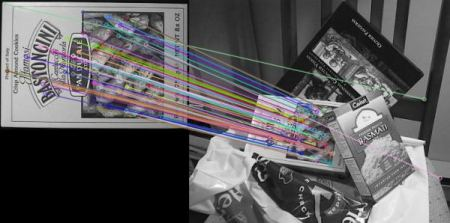
\includegraphics[width=.6\textwidth]{images/01/sift.jpeg}
    \caption{Korešpondencia lokálnych príznakou použítím metódy SIFT \cite{sift-img}.}
    \label{img:sift}
\end{figure}

Nakoniec v poslednom kroku je použitý klasifikátor, napríklad \textit{support vector machine (SVM)} \cite{SVM} alebo \textit{Adaptive Boosting (Adaboost)} \cite{Adaboost} na určenie finálnej identifikácie a lokalizácie objektu.
TODO prepojiť obrázok s textom. Povedať jednu-dve vety o SVM. Adaboost môže isť ptm preč.
\begin{figure}[H]
    \centering
    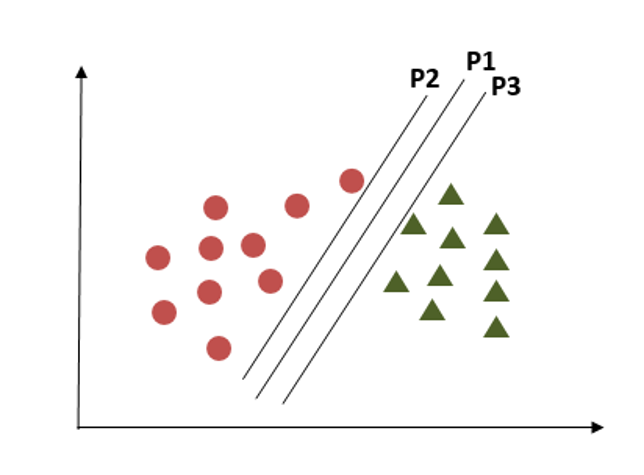
\includegraphics[width=.6\textwidth]{images/01/svm.png}
    \caption{Todo, SVM, vymeniť/preložiť obrázok.}
    \label{img:svm}
\end{figure}

Pri detekcii treba brať do úvahy viacero možných problémov, ktoré v nietorých prípadoch môžu predstavovať neprekonateľné prekážky pre tradičné metódy. Častými problémami je oklúzia, osvetlenie, deformácia, variácia pohľadu a variácia objektu v rámci jednej triedy. Neurónové siete majú väčšiu presnosť detekcie aj pri takýchto problémoch, čím sú oveľa robustnejšie než tradičné metódy a preto sú dobrou voľbou nielen pre našu prácu  ale aj pre množstvo použití v reálnom živote.

\subsection{Detekcia reklám}

Neurónové siete sa na detekciu objektov využívajú už desaťročia a nie je prekvapením, že sú často používané aj pri pozorovaní dopravy. Detekcia áut, chodcov, dopravných a poznávacích značiek je z pohľadu pozorovania dopravy fundamentálna úloha, ktorá je spracovaná v mnohých prácach. Našli sme aj viaceré publikácie priamo zamerané na detekciu reklamných plôch, ktorými sa možno inšpirovať a porovnať.

Autori práce \cite{SSD-YOLO} porovnávajú dva detektory objektov, \textit{Single Shot MultiBox Detector (SSD)} a \textit{You Only Look Once (YOLOv3)}. Oba detektory boli najskôr trénované na \textit{COCO} databáze \cite{Coco} a potom na sade obrázkov zobrazujúce bilbordy. V obidvoch prípadoch modely dosahujú dobré výsledky pre rôzne veľkosti reklám za rôznych svetelných podmienok s komplexným pozadím. Výsledky z experimentu naznačujú, že SSD je presnejší v tom zmysle, že robí menej chýb pri identifikácii výskytu reklamy. Na druhej strane YOLOv3 dokáže vyhodnotiť výsledok za kratší čas, ale dopúšťa sa väčšej chybovosti označovaním falošných výskytov. Čiastočne by to mohla vybalansovať zmena prahu istoty pre označenie výskytu, čo ale v práci nebolo testované. Na obrázku \ref{img:ssd-yolo} vidno, že YOLOv3 má vyššie hodnoty pre istotu, preto by zrejme potreboval zvýšiť prah na určenie detekcie.
\begin{figure}[H]
    \centering
    \includegraphics[width=.6\textwidth]{images/01/ylssd.png}
    \caption{Histogramy príslušných hodnôt istoty detekcie pre SSD a YOLOv3 \cite{SSD-YOLO}.}
    \label{img:ssd-yolo}
\end{figure}

%\begin{figure}[H]
%    \centering
%    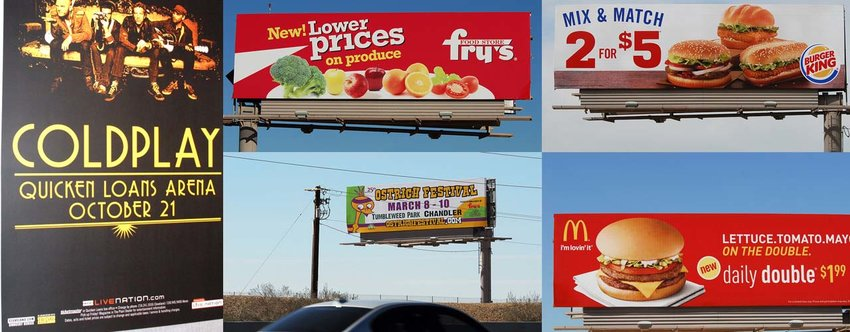
\includegraphics[width=.6\textwidth]{images/01/coco-ads.png}
%    \caption{Ukážka vzorových dát z COCO databázy}
%    \label{img:coco}
%\end{figure}

V práci \cite{Hossari} na detekciu reklám autori navrhli \textit{Advert detection model (ADNet)} inšpirovaný \textit{VGG} architektúrou \cite{simonyan2015deep}. Rozdiel voči VGG je v tom, že ADNet preskakuje päť vrstiev zo začiatku a tri z konca. Na koniec pridáva tri plne prepojené vrstvy a hneď po prvej sa aktivuje \textit{dropout} s 50\% stratou prepojenia medzi dvoma uzlami. Navrhnutú sieť trénovali na databáze \textit{Mapillary Vistas} \cite{Mapillary}. Výsledky práce uvádzajú iba v presnosti klasifikácie (snímok s reklamou alebo snímok bez reklamy) na úrovni 94\%. Tiež uvádzajú, že počas testovania vedia každú snímku z videa vyhodnotiť za 54ms.

V práci \cite{GeoTag} bola ako základ použitá architektúra AlexNet \cite{AlexNet}, ktorej cieľom bolo vyhodnotiť nahrávané video v reálnom čase a nahlásiť polohu reklamy s jej obsahom. Výsledky na vlastnej databáze dosiahli významne menšiu presnosť a to najmä na detekcii menších reklamných plôch. Autori opisujú vývoj trénovania skúšaním rôznych parametrov. Nakoniec dosiahli úspešnosť tréningu 92.7\%, ale výsledky na testovacích dátach dopadli približne o 20\% horšie, čo je zjavne spôsobené prehnaným trénovaním. Detekcie reklám boli ďalším procesom rozdelené do kategórií ako nehnuteľnosti, kampaň, produkty a mnohé iné, avšak bližšie výsledky v práci neboli uvedené.

\section{Významnosť reklám}

Pozornosť vodiča je kritickým problémom, ktorému sa v posledných rokoch venuje veľká pozornosť. Je nevyhnutné, aby vodiči zostali počas jazdy sústredení  a aby sa vyhli nebezpečným situáciám na ceste. Ľudská pozornosť je častokrát ľahko ovplyvniteľná a existuje veľa rušivých prvkov, ktoré môžu odviesť pozornosť vodiča. Jedným z takýchto rozptýlení môže byť reklama, ktorá má potenciál odvrátiť pozornosť vodičov od cesty. Štúdie ukázali, že aj chvíľkové rozptýlenie môže mať pri šoférovaní vážne následky. Napríklad vodič, ktorý v meste odtrhne oči od vozovky len na dve sekundy, aby si prečítal obsah reklamy prejde vzdialenosť približne 28 metrov. Keď sa to skombinuje so situáciou, kedy vodič musí reagovať na náhlu zmenu v premávke, nemusí mať dostatok času odvrátiť nehodu.

Všetky nájdené štúdie, ktoré pozorovali účinky reklamy na vodiča používali eyetracker zariadenie na sledovanie pohľadu vodiča. Niektoré okrem toho merali rýchlosť vozidla, kognitívne funkcie z EEG zariadenia alebo aplikovali metódu “Wiener Fahrprobe” \cite{WF} na pozorovanie vodičovho správania, ktorá spočíva v zaradení dvoch ďalších sledovateľov do vozidla a následnom sledovaní zmeny v šoférovaní vodiča.  Je dôležité povedať, že štúdie neboli konzistentné a líšili sa v mnohých dôležitých veciach. Približne polovica štúdií zbierala dáta z reálneho prostredia a druhá polovica využívala namiesto reálnej jazdy simulátory v rôznych podmienkach.

Vplyv na správanie vodiča závisí od charakteristiky reklamy a od samotného vodiča. U mladých \cite{stavrinos2016visual} a starších vodičov \cite{belyusar2016field, EDQUIST2011619} boli identifikované dlhšie fixácie na reklamy, čo viedlo k väčšej chybovosti než pre zvyšok vodičov. Práca \cite{horberry200813} pridáva tvrdenie, že starší vodiči jazdili pomalšie na úsekoch s veľkou hustotou reklám. Podobné výsledky sa ukázali aj pri neskúsených vodičov. V práci \cite{bendak2010role} zistili, že vodič prechádzajúci okolo reklamy má mierne problémy s držaním vozidla v správnom jazdnom pruhu a v križovatkách. Pri pozorovaní rozdielov medzi pohlavím sa v žiadnej práci neuvádzajú významné rozdiely.

\subsection{Charakteristiky reklám}

Podľa prečítaných prác by sa charakteristika reklám dala rozdeliť  na základe nasledujúcich troch parametrov.

\subsubsection{Typ reklamy}

Viaceré práce ukazujú, že elektronické bilbordy dosahujú dlhší pohľad v porovnaní s tradičnou reklamou, ktorá nevyžaruje svetlo \cite{OVIEDOTRESPALACIOS201985, beijer, brome}. Naopak v práci \cite{n1} toto tvrdenie nebolo potvrdené, pretože sa nenašli žiadne zásadne rozdiely medzi tradičnými a elektronickými bilbordmi. Experiment v práci \cite{brome} ukazuje, že elektronické bilbordy, ktoré v krátkych intervaloch striedajú obsah priťahujú vodičovú pozornosť častejšie, ale celková dĺžka fixácia nie je výrazne odlišná. Autori sa v prácach \cite{mollu2018driving} a \cite{beijer} zhodujú s tým, že vysoká svietivosť v prípade elektronickej reklamy môže byť príčinou dopravnej nehody, nakoľko najdlhšie ovplyvnia správanie vodiča. Potvrdili to aj účastníci experimentu svojimi názormi v dotazníku, ktorý vyplnili krátko po ukončení jazdy. Obzvlášť veľkú pozornosť pútajú elektronické bilbordy s video obsahom. Práve takýto typ reklamy je kvôli priemernej dĺžke fixácií najnebezpečnejší \cite{yellappan2016exposure, smiley2005traffic}.

\subsubsection{Umiestnenie reklamy}

Dosah reklamy významne závisí aj od jej umiestenia. Reklamy situované na vodičovej strane cesty zaznamenali viacej fixácii než na opačnej strane cesty. Predpoklad, že výška umiestnenia reklamy predĺži trvanie fixácie bol negatívne potvrdený v práci \cite{costa} a \cite{crundall}. Autori zistili, že vodiči sa viac pozerali na reklamy na úrovni cesty než na reklamy vyvýšené tri a viac metrov nad zemou. Výnimkou sú prípady, kedy vodiči cielene vyhľadávajú reklamy, vtedy sa obzerajú viac do výšky. Okrem toho niektoré práce brali do úvahy uhol reklamnej plochy \cite{zalesinska2018impact}, náročnosť dopravného úseku, typ prostredia a jeho komplexnosť \cite{costa, mollu2018driving} pričom sa ukázalo, že všetky tieto prvky do istej miery vplývajú na sledovanosť reklamy.

\subsubsection{Obsah reklamy}

Poslednou dôležitou charakteristikou reklamy je jej obsah. Štúdie \cite{harasimczuk2021longer, meuleners2020identifying} potvrdzujú predpoklad, že reklamy s dlhším textom dosahujú dlhšie fixácie. To takisto platí pre reklamy so sexuálnym podtónom \cite{MaliszewskiNorbert2019Iosa} a pre reklamy, na ktorých sa nachádza ľudská bytosť \cite{tarnowski2017roadside}. Zároveň platí, že čím je reklama zložitejšia, tým dlhšie sa na ňu vodič pozerá \cite{marciano2017effect}. Skúmaný bol aj obsah reklamy, ktorý u vodiča vyvoláva negatívne emócie \cite{chan2013emotional}. Zistilo sa, že takisto zapríčiňuje dlhšie fixácie a zároveň vedie k zníženiu rýchlosti. Okrem toho dotazníky vyplnené vodičmi po jazde ukázali, že negatívnu reklamu si vodiči zapamätajú najviac.

% \section{Mapa význačností}
%
% Z pohľadu počítačového videnia existujú viaceré metódy, ktoré detekujú významné oblasti v scénach. Ako prvý najvplyvnejší pokus v tejto oblasti urobili Christof Koch a Shimon Ullman  \cite{Itti}. Navrhli, aby sa rôzne vizuálne prvky, ktoré prispievajú k výberu pozornosti (napríklad farba, orientácia, pohyb a iné), skombinovali do jedinej topograficky orientovanej mapy. Integráciou normalizovaných informácií jednotlivých vizuálnych prvkov vzniká mapa význačnosti.
%
% Najrozsiahlejší dataset na vyhodnocovanie mapy význačností je SALICON \cite{SALICON} a MIT300 \cite{MIT300}. Na oboch datasetoch v súčastnosti dosahuje najlepšie výsledky TranSalNet \cite{TranSalNet}. Model integruje komponenty z transformátorov do CNN na zachytenie kontextových vizuálnych informácií s dlhým dosahom. Experimentálne výsledky ukazujú, že transformátory poskytujú pridanú hodnotu ku predikcii význačnosti.
%
% \subsection{Predikcie pohľadu vodiča}
%
% Mapa význačnosti pre video je doposiaľ menej preskúmaná, ale pribúda čoraz viac prác, ktoré prinášajú významné pokroky v tejto oblasti. Pomocou mapy význačností vo videu sa dá predikovať pohľad vodiča pri riadení vozidla. Skupina autorov navrhla model \cite{FoA} založený na viac vetvovej hlbokej architektúre, ktorá integruje tri zdroje informácií: RGB snímku, optický tok (optical flow) a sémantickú segmentáciu. Na tréning a testovanie použili DR(eye)VE dataset, ktorý obsahuje menej interakcií s ostatnými účastníkmi cestnej premávky. Navrhnutý model mali vysokú tendenciu predikovať fixáciu na stred snímky, podobne ako ostatné modely trénované na tomto datasete.
%
% V ďalšej práci \cite{BDDA} bolo navrhnuté použitie metódy Human Weighted Sampling (HWS), ktorá využíva správanie ľudského pohľadu na identifikovanie dôležitých údajov z jazdy a prikladá im rôznu váhu počas tréningu modelu. Výsledkom bol model predikcie, ktorý demonštruje sofistikované správanie, ako je napríklad sledovanie ľudí na prechode pre chodcov, pričom potláča pohľad na chodcov kráčajúcich bezpečne po chodníku. Použitý dataset obsahoval primárne také situácie, kedy bolo vozidlo nútené zastaviť.